\subsection{Criterios para asignación de polos en lazo cerrado}

Sea el sistema
\[(1)
    \left\{
        \begin{array}{lll}
            \dot{x}(t) = Ax(t) + Bu(t) \\
            y(t) = Cx(t)
        \end{array}
    \right.
\]

hay dos casos al momento de obtener la función de transferencia

\begin{itemize}
    \item a) Sin ceros
    \[
        \frac{x(s)}{y(s)} = \frac{b}{s^{n} + \tilde{a}_{1}s^{n-1} + \ldots + \tilde{a}_{n}} = \frac{b}{(s-\mu_{1})(s-\mu_{2})\ldots(s-\mu_{n})}
    \]
    \item b) Con ceros y polos
    \[
        \frac{x(s)}{y(s)} = \frac{(s-q_{1}) (s-q_{2}) \ldots (s-q_{m})}{(s-\mu_{1})(s-\mu_{2})\ldots(s-\mu_{n})} \;\; \text{con \( m < n \)}
    \]
    
\end{itemize}

La función de transferencia se aproxima a un sistema de segundo orden, de la forma
\[
    \frac{y(s)}{x(s)} = \frac{W_{n}}{s^{2} +2 \xi W_{n}s + W_{n}^{2} } \;\; (2)
\]

Donde 
\[
    \begin{split}
        \xi & : \text{amortiguamiento} \\
        W_{n} & : \text{frecuencia natural}
    \end{split}
\]

\begin{figure}[h!]
    \centering
        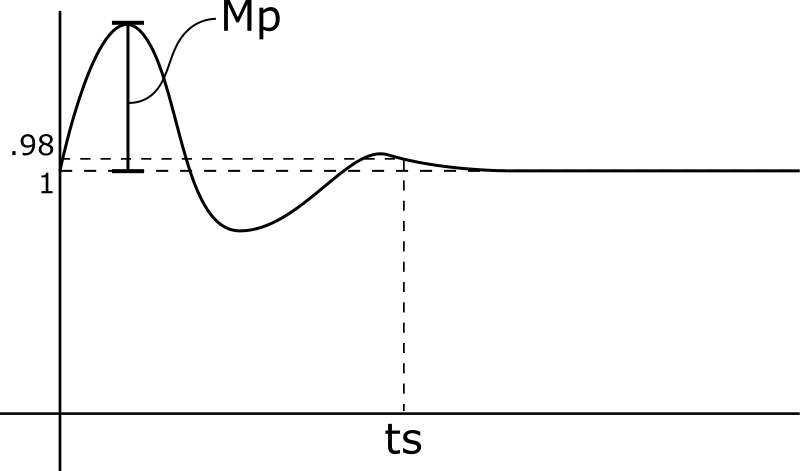
\includegraphics[scale=0.25]{Control de Sistemas Mecatronicos Figuras/18 Sistema de Segundo Orden.png}
        \caption{Sistema de segundo orden}
\end{figure}

Entonces se define el máximo sobre impulso
\[
    M_{p} = e^{^{- \xi \pi}/_{\sqrt{1 - \xi^{2}}}}
\]

Tiempo de asentamiento: tiempo para mantenerse alrededor del valor final
\[
    \begin{split}
        t_{s} = \frac{4}{\xi W_{n}} \;\; \text{Criterio del 2\%} \\
        t_{s} = \frac{3}{\xi W_{n}} \;\; \text{Criterio del 5\%}
    \end{split}
\]

La ecuación (2) se resuelve 
\[
    \text{polos dominantes} < S_{1,2} = -\xi W_{n} \pm W_{n}(\sqrt{\xi^{2} - 1})
\]

Polos no dominantes: deben de estar mas alejados de los dominantes, al menos 5 veces en valor absoluto del polo dominante

Para el caso b) eliminar los ceros con los polos, tal que
\[
    \mu_{3} \approx q_{1}, \mu_{4} \approx q_{2}, \ldots,
     \mu_{n+m} \approx q_{m} 
\]